\documentclass[a4paper,12pt]{article}
\usepackage{amsmath, amsthm, amssymb}
\usepackage{tikz} % 添加绘图
\usepackage{tabularx}
\usepackage{enumitem}
\usepackage{fancyref}

\usepackage[top=1in,bottom=1in,left=1in,right=1in]{geometry} % 用于设置页面布局
\usepackage{xeCJK} % 用于使用本地字体
\usepackage[super, square, sort&compress]{natbib} % 处理参考文献
\usepackage{titlesec, titletoc} % 设置章节标题及页眉页脚
%\usepackage{xCJKnumb} % 中英文数字转换
\usepackage{amssymb}
\usepackage{amsmath} % 在公式中用\text{文本}输入中文
\usepackage{diagbox}
\usepackage{multirow} % 表格中使用多行
\usepackage{booktabs} % 表格中使用\toprule等命令
\usepackage{rotating} % 使用sidewaystable环境旋转表格
\usepackage{tabularx}
\usepackage{graphicx} % 处理图片
\usepackage{footnote} % 增强的脚注功能,可添加表格脚注
\usepackage{threeparttable} % 添加真正的表格脚注,示例见README
\usepackage{hyperref} % 添加pdf书签

\usepackage{tikz}
\usetikzlibrary{shapes,arrows,shadows}

% 字体设置
\setmainfont{Times New Roman}
\setsansfont[Scale=MatchLowercase,Mapping=tex-text]{PT Sans}
\setmonofont[Scale=MatchLowercase]{PT Mono}
\setCJKmainfont[ItalicFont={Kaiti SC}, BoldFont={Heiti SC}]{Songti SC}
\setCJKsansfont{Heiti SC}
\setCJKmonofont{Songti SC}
% \setCJKmainfont[BoldFont={FZXiaoBiaoSong-B05S}]{Songti SC}
% \setCJKfamilyfont{kai}[BoldFont=Heiti SC]{Kaiti SC}
% \setCJKfamilyfont{song}[BoldFont=Heiti SC]{Songti SC}
% \setCJKfamilyfont{hei}[BoldFont=Heiti SC]{Heiti SC}
% \setCJKfamilyfont{fsong}[BoldFont=Heiti SC]{Songti SC}
% \newcommand{\kai}[1]{{\CJKfamily{kai}#1}}
% \newcommand{\hei}[1]{{\CJKfamily{hei}#1}}
% \setromanfont[Mapping=tex-text]{TeXGyrePagella}
% \setsansfont[Scale=MatchLowercase,Mapping=tex-text]{TeXGyrePagella}
% \setmonofont[Scale=MatchLowercase]{Courier New}
%%设置常用中文字号,方便调用
\newcommand{\erhao}{\fontsize{22pt}{\baselineskip}\selectfont}
\newcommand{\xiaoerhao}{\fontsize{18pt}{\baselineskip}\selectfont}
\newcommand{\sanhao}{\fontsize{16pt}{\baselineskip}\selectfont}
\newcommand{\xiaosanhao}{\fontsize{15pt}{\baselineskip}\selectfont}
\newcommand{\sihao}{\fontsize{14pt}{\baselineskip}\selectfont}
\newcommand{\xiaosihao}{\fontsize{12pt}{\baselineskip}\selectfont}
\newcommand{\wuhao}{\fontsize{10.5pt}{\baselineskip}\selectfont}
\newcommand{\xiaowuhao}{\fontsize{9pt}{\baselineskip}\selectfont}
\newcommand{\liuhao}{\fontsize{7.5pt}{\baselineskip}\selectfont}

% 章节标题显示方式及页眉页脚设置
% \item xCJKnumb是自己额外安装的包
% \item titleformat命令定义标题的形式
% \item titlespacing定义标题距左、上、下的距离
\titleformat{\section}{\raggedright\large\bfseries}{\thesection}{1em}{}
\titleformat{\subsection}{\raggedright\normalsize\bfseries}{\thesubsection}{1em}{}
\titlespacing{\section}{0pt}{*0}{*2}
\titlespacing{\subsection}{0pt}{*0}{*1}
% 由于默认的2em缩进不够,所以我手动调整了,但是在windows下似乎2.2就差不多了,或者是article中没有这个问题
\setlength{\parindent}{2.2em}

% 设置表格标题前后间距
\setlength{\abovecaptionskip}{0pt}
\setlength{\belowcaptionskip}{0pt}


\renewcommand{\refname}{\bfseries{参~考~文~献}} %将Reference改为参考文献(用于 article)
% \renewcommand{\bibname}{参~考~文~献} %将bibiography改为参考文献(用于 book)
\renewcommand{\baselinestretch}{1.38} %设置行间距
\renewcommand{\figurename}{\small\ttfamily 图}
\renewcommand{\tablename}{\small\ttfamily 表}

\setlength{\parindent}{0em}
\setlength{\parskip}{0.5em}

\newtheorem{definition}{定义}
\newtheorem{lemma}{引理}
\newtheorem{proposition}{命题}
\newtheorem{program}{程序}
\newtheorem{convention}{约定}
\renewcommand*{\proofname}{证明}

\title{关于理解伴随的几种思路}
\author{苑明理}
\date{2018年12月}

\begin{document}

\maketitle{}

\renewcommand\contentsname{目录}
\setcounter{tocdepth}{2}
\tableofcontents

\newpage

\section{问题的提出}

伴随出现在许多数学领域,它在最优控制、敏感分析、变分同化中都扮演了重要的角色。近来在深度学习同微分方程结合的方向上,人们也发现了伴随的重要价值。
在学习、理解伴随概念的过程中,我们整理出在相关领域文献里三种推导伴随的思路,并认为这些思路应该是统一的。

\subsection{基本定义及几何解释}

\begin{definition}
\label{d0}
两个向量空间 $X$、$Y$ 通过一个到域 $ F $ 的双线性映射 $ \langle , \rangle : X \times Y \to F $ 构成一个对偶系统 $ \langle X, Y \rangle $。
\end{definition}

对偶系统的一个例子是 $ E^3 $ 和其上的一个标架系统 $ (x, y, z) $ 。借鉴这个例子,我们做如下约定:

\begin{convention}
称对偶系统 $ \langle X, Y \rangle $ 中的 $ X $ 为底空间, $ Y $ 为标架空间,$ \langle x, y \rangle $ 的值为坐标。
\end{convention}

在日常生活中,我们都有如下的经验

\begin{figure}[ht]
\centering
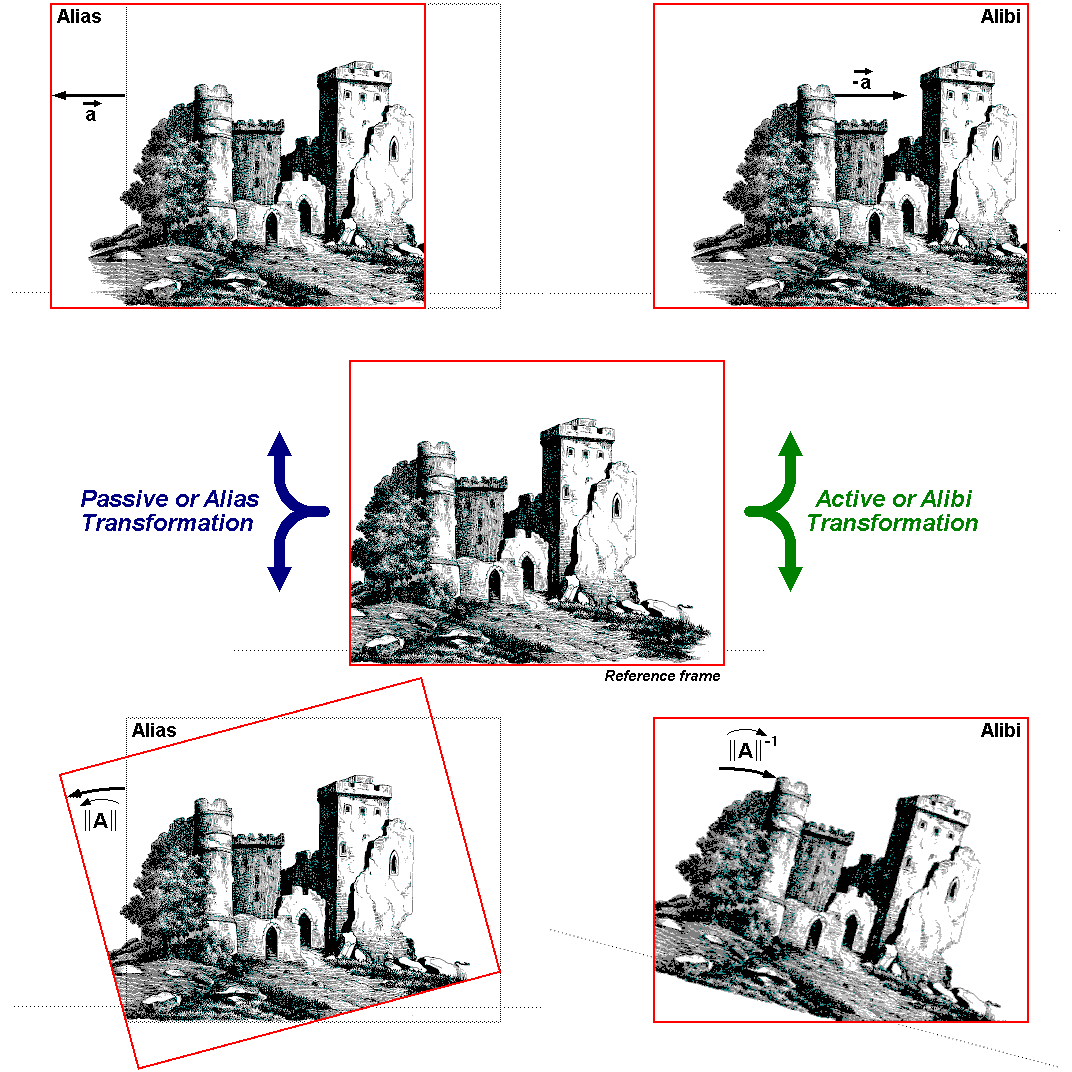
\includegraphics[width=3.5in]{images/adjoint/alias_and_alibi.png}
\caption{两对互为伴随的映射,图片来自维基}
\end{figure}

仔细体会上图的内涵,我们就到达了伴随这一概念。

\begin{definition}
\label{d1}
考虑两个对偶系统 $ \langle X_1, Y_1 \rangle $ 和 $ \langle X_2, Y_2 \rangle $ ,两个算符 $ A : X_1 \to X_2$ 和  $B : Y_2 \to Y_1 $ 称为互为伴随的,
当且仅当,对任意的 $ \phi \in X_1 $ 和 $ \psi \in Y_2 $ 下式得到满足:$$ \langle A \phi, \psi \rangle = \langle \phi, B \psi \rangle $$
\end{definition}

\subsection{几种约束优化问题}

一般等值的约束优化问题可以写成

$$
\begin{array}{rcll}
\min &~& J(\mathbf{x}) & \\
\mathrm{s.t.} &~& g(\mathbf{x}) = \mathbf{c}
\end{array}
$$

几何上看,就是在约束面上寻求 $ J $ 的最小值。非常直观的,极值发生在 $ J $ 的梯度同约束面彼此垂直,或者说 $ J $ 的等值线同约束面相切的情况下。
极值的求解是通过 Lagrange 乘子的方法来做的。

\begin{figure}[ht]
\centering
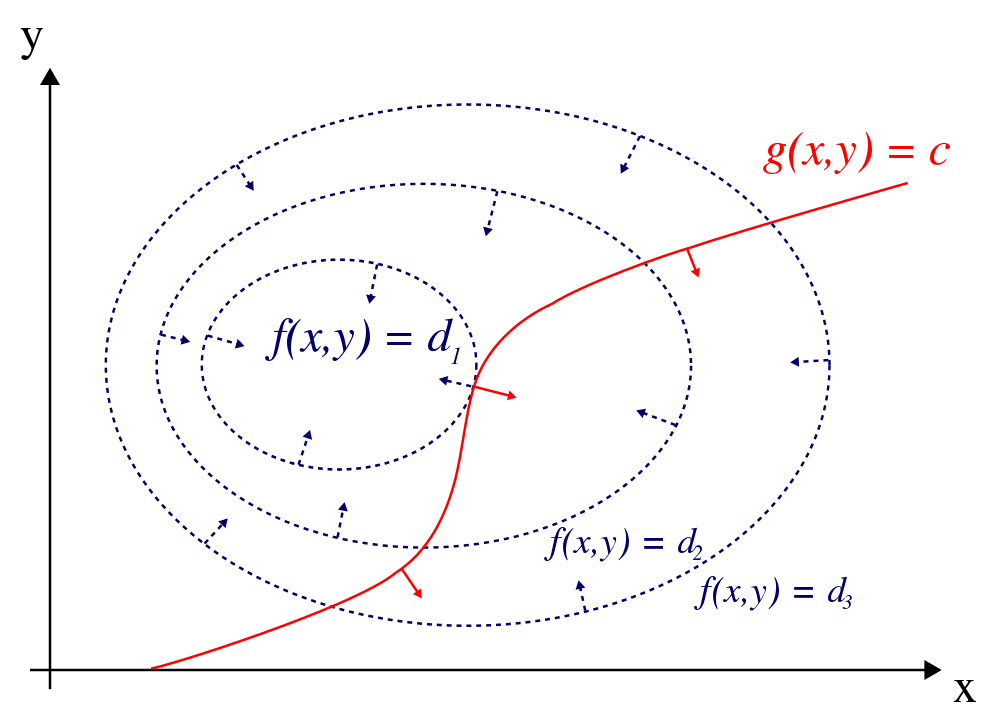
\includegraphics[width=3.5in]{images/adjoint/lagrange_multiplier.png}
\caption{一般的等值约束最优化问题,图片来自维基}
\end{figure}

在很多应用情况下,约束是由一个含时演化系统给出,如

含时常微分方程:

$$
\frac{d\mathbf{x}}{dt} = f(\mathbf{x}, t; \theta)
$$

或者,含时偏微分方程组:

$$
\frac{\partial x_i}{\partial t} = f_i \left( x_1, \ldots x_n; u, \frac{\partial u}{\partial x_1}, \ldots \frac{\partial u}{\partial x_n}; \frac{\partial^2 u}{\partial x_1 \partial x_1}, \ldots \frac{\partial^2 u}{\partial x_1 \partial x_n}; \ldots ; u; \theta \right), i \in \{1, \ldots , n\}
$$

上述两种情况,都可以由算子半群给予统一的描述。

针对不同的具体问题, $ J $ 的给出略有不同,我们关心的情况包括:最优控制、资料同化和参数学习。

\subsubsection{最优控制}

为了简化,我们仅仅考虑最优控制的一种可能的情形,受演化方程 $ f $ 控制的一个过程,
我们需要调整边界上的控制变量 $ \mathbf{u} = \mathbf{y}_{\partial} $ ,使得在终止时刻的计算值 $ \mathbf{y}_1 = \mathbf{y}(\mathbf{x}, 1)$ 同目标值 $ \mathbf{y}_1^o $ 之间的误差最小。

$$
\begin{array}{rcll}
\min &~& J(\mathbf{y_1}, \mathbf{y}_1^o, \mathbf{u}) & \\
\mathrm{s.t.} &~& \dot{\mathbf{y}} = f(\mathbf{x}, t; \theta) & (\mathbf{x}, t) \in \Omega \times [0, 1] \\
&~& \mathbf{y} = u(\mathbf{x}, t; \theta) & (\mathbf{x}, t) \in \partial \Omega \times [0, 1] \\
&~& \mathbf{y}(\mathbf{x}, 0) = \mathbf{y}_0(\mathbf{x}) & \mathbf{x} \in \Omega
\end{array}
$$

其中的 $ J $ 由下式给出:

$$
J(\mathbf{y_1}, \mathbf{y}_1^o, \mathbf{u}) = \frac{1}{2} \int\limits_{\Omega}|\mathbf{y_1} - \mathbf{y_1^o}|^2dx +  \frac{\lambda}{2} \int\limits_{0}^{1}\int\limits_{\partial \Omega} |\mathbf{u}|^2 dS(x) dt
$$


\subsubsection{资料同化}

从数学的观点看,数值天气预报是求解一个偏微分方程的初值问题。但受限于观测,我们无法直接给出一个确切的初值,因此需要通过一定技术手段来确定初始值。
本文我们仅讨论四维变分同化技术里基本原理的简化版本。

无法得到确切初值的原因首先是因为观测是不完整的,某个时间只有某些地区是有观测的。我们把有观测的区域定义成一个可以在空间上积分的特征函数:

$$
O(\mathbf{x}, t) = \begin{cases}
1, & \text{if }\mathbf{x} \text{ is observable at t} \\
0, & \text{if }\mathbf{x} \text{ is not observable at t}
\end{cases}
$$

另外一个原因是因为观测方法的局限,观测量不直接是大气状态场。我们把观测定义成一个空间位置 $ \mathbf{x} $ 和大气状态 $ \mathbf{y} $ 的函数 $ M(\mathbf{x}, \mathbf{y}) $

受演化方程 $ f $ 控制的一个过程,给定一个初始时刻的背景场 $ \mathbf{y}_0^b = \mathbf{y}(\mathbf{x}, 0) $ ,它会导致终止时刻的计算场 $ \mathbf{y}_1 = \mathbf{y}(\mathbf{x}, 1) $ ,
也会得到一个反演的观测场 $ \mathbf{m}_1 = M(\mathbf{x}, \mathbf{y}_1) O(\mathbf{x}, 1) $。

我们需要调整控制变量 $ \mathbf{u} = \mathbf{y}_0 - \mathbf{y}_0^b $ ,它的变化会使反演观测场 $ \mathbf{m}_1 $变化,
我们的目标是使得终止时刻的反演观测场 $ \mathbf{m}_1 $ 同终止时刻的实际观测场 $ \mathbf{m}_1^o $ 之间的误差最小。

$$
\begin{array}{rcll}
\min &~& J(\mathbf{m_1}, \mathbf{m}_1^o, \mathbf{u}) & \\
\mathrm{s.t.} &~& \dot{\mathbf{y}} = f(\mathbf{x}, t; \theta) & (\mathbf{x}, t) \in \Omega \times [0, 1] \\
&~& \mathbf{y} = g(\mathbf{x}, t; \theta) & (\mathbf{x}, t) \in \partial \Omega \times [0, 1] \\
\end{array}
$$

其中的 $ J $ 由下式给出:

$$
J(\mathbf{m_1}, \mathbf{m}_1^o, \mathbf{u}) = \frac{1}{2} \int\limits_{\Omega}|\mathbf{u}|^2 dx + \frac{\lambda}{2} \int\limits_{\Omega}|\mathbf{m}_1 - \mathbf{m}_1^o|^2 dx
$$

\subsubsection{参数学习}

(先用学习的标准语言来陈述,再转化到最优化的语言)

受演化方程 $ f $ 控制的一个过程,给定一个初始值 $ \mathbf{y}_0 $ ,需要调整参数 $ \theta $ ,使得在终止时刻的计算值 $ \mathbf{y_1} $ 同观测值 $ \mathbf{y}_1^o $ 之间的误差最小。

$$
\begin{array}{rcll}
\min &~& J(\mathbf{y_1}, \mathbf{y}_1^o) & \\
\mathrm{s.t.} &~& \dot{\mathbf{y}} = f(\mathbf{x}, t; \theta) & (\mathbf{x}, t) \in \Omega \times [0, 1] \\
&~& \mathbf{y} = g(\mathbf{x}, t; \theta) & (\mathbf{x}, t) \in \partial \Omega \times [0, 1] \\
&~& \mathbf{y}(\mathbf{x}, 0) = \mathbf{y}_0(\mathbf{x}) & \mathbf{x} \in \Omega
\end{array}
$$

\section{几种伴随的推导思路}

我们尝试把文献中的不同推导思路应用到一个一维平流扩散方程上的最优控制问题上:

$$
\begin{array}{rcll}
\min &~& (y_1 - y_1^o)^2 & \\
\mathrm{s.t.} &~& \dot{y} = y_{xx} - y_x & x \in [-1, 1], t \in [0, 1]\\
&~& y(-1, t) = u(t) & t \in [0, 1]\\
&~& y(+1, t) = v(t) & t \in [0, 1]\\
&~& y(x, 0) = y_0(x) & x \in [-1, 1]
\end{array}
$$

其中的 $ u $ 和 $ v $ 是控制变量。

\subsection{第一种推导思路}

\subsection{第二种推导思路}

\subsection{第三种推导思路}

\section{进一步讨论}

\subsection{三种思路的关系}

\subsection{伴随方法的优点}

\end{document}
